\subsection{Filtro passa-banda de Rauch} \label{filtro_rauch}

\subsubsection{Análise Teórica}

% a imagem do esquema eletrico fo filtro passa-banda de rauch deve ter a legenda 

Na segunda parte da Sessão 2, temos como objetivo analisar um filtro passa-banda de Rauch a partir de uma montagem feita numa \textit{breadbord}. Posteriormente é adicionado um circuito atenuador entre o osciloscópio e o filtro passa-banda. Temos que determinar a função de transferência de um filtro passa-banda de Butterworth de 2ª ordem, com frequência central $f_o = 1$ kHz, largura de banda $B =250$ Hz e com ganho $G_{f_0} = 24$ dB na frequência central. A modelação de um filtro passa-banda pela aproximação de Butterworth é feita obtendo inicialmente uma aproximação para um filtro passa-baixo sendo depois feita uma transformação para passar o filtro de passa-baixo para passa-banda.\par
Em primeiro lugar, temos que garantir que as especificações dadas permitem modelar um filtro com simetria geométrica, logo podemos escrever o seguinte sistema de equações:
\begin{equation*}
    \begin{cases}
    {\omega_0}^2= \omega_{p1} \omega_{p2} \\
    B=\omega_{p2}- \omega_{p1}
    \end{cases} \Leftrightarrow
    \begin{cases}
    \omega_{p1}= 5546.68 rad/s \\
    \omega_{p2}=7117.48 rad/s \: .
    \end{cases}
\end{equation*}

De seguida, para $A_p = \sqrt{2} \approx 3$ dB, pela definição de frequência de corte, podemos retirar que $\epsilon = 1$. Uma vez que a ordem do filtro duplica quando é feita a transformação do filtro passa-baixo para passa-banda, a ordem do filtro passa-baixo original é $n=1$. Pelas tabelas de Butterworth retiramos a expressão de $H(\hat{S})$, podendo escrever, assim, a sua função de transferência 
\begin{equation}
\label{eq:tf_}
    T(\hat{S})= \frac{K}{H(\hat{S})}=\frac{K}{\hat{S} + 1}\:.
\end{equation}
Sabendo que
\begin{equation*}
    \hat{S} = \epsilon \frac{s^2 + \omega_0^2}{B s}
\end{equation*}
podemos substituir na função de transferência \eqref{eq:tf_} obtendo a função de transferência para um filtro de passa-banda de 2ª ordem
\begin{equation}
    T_{BP}(s)=\frac{KBs}{s^2 + Bs + \omega_0^2} \: .
    \label{eq:tbp}
\end{equation}
Porém, temos ainda que garantir o ganho de 24dB para a frequência central, logo
\begin{equation*}
    |T(j\omega_0)|= G_{f_0} \Leftrightarrow  \left|\frac{KBs}{s^2 + Bs + \omega_0^2}\right|= 10 ^{\frac{24}{20}} \Leftrightarrow |K|\approx15.85
\end{equation*}
A função de transferência de um filtro passa-banda de 2ª ordem, com as especificações indicadas, é definida por
\begin{equation}
    \label{eq:tf_butter}
    T_{BP}(s)=\frac{2.49 \times 10^4 s}{s^2 + 1571s + 3.948 \times 10^7} \: .
\end{equation}
A partir da função de transferência, podemos facilmente representar os diagramas de bode para amplitude e para a fase, apresentados na Fig. \ref{fig:bode_bp}.
\begin{figure}[ht]
    \centering
    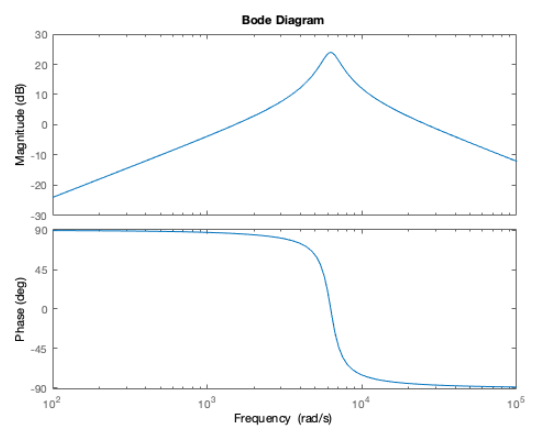
\includegraphics[width = 0.7 \textwidth]{Imagens/bode_bp.png}
    \caption{Diagramas de Bode de amplitude e fase para a função de transferência \eqref{eq:tf_butter}.}
    \label{fig:bode_bp} 
\end{figure}

\subsubsection{Trabalho Experimental}
Procedeu-se à montagem do filtro passa-banda de Rauch de acordo com o esquema apresentado na Fig.~\ref{fig:passa_banda_Rauch}. Foi aplicado na entrada do filtro um sinal sinusoidal com uma amplitude pequena, ajustada aquando da atividade laboratorial, de forma a que o AmpOp não saturasse. Visto que o filtro é passa-banda e inversor, à frequência central observa-se uma diferença de fase de $180 \degree$ e às frequências de corte uma diferença de fase de $180\degree \pm 45 \degree$, entre os sinais de saída e de entrada.  Fazendo variar a frequência da onda sinusoidal à entrada do filtro até se obterem as diferenças de fase mencionadas anteriormente foram determinadas experimentalmente a frequências de corte ($f_{c_i}$ e $f_{c_s}$) e a frequência central do filtro ($f_0$), apresentadas na Tabela \ref{tb:freqsRauch}, bem como a largura de banda ($B$) e o ganho à frequência central ($G_{f_0}$). As ondas observadas nos osciloscópio para determinar estes valores estão apresentadas na Fig. \ref{fig:ocsl_freqs}. No caso da frequência central experimental, $f_0$, para uma diferença de potencial pico-a-pico da sinusóide de entrada de $460$mV obteve-se uma tensão de $6.80$V pico-a-pico na saída. É de salientar que todas as grandezas foram medidas no osciloscópio, que permite uma maior exatidão na sua determinação.

\begin{figure}[ht]
    \centering
    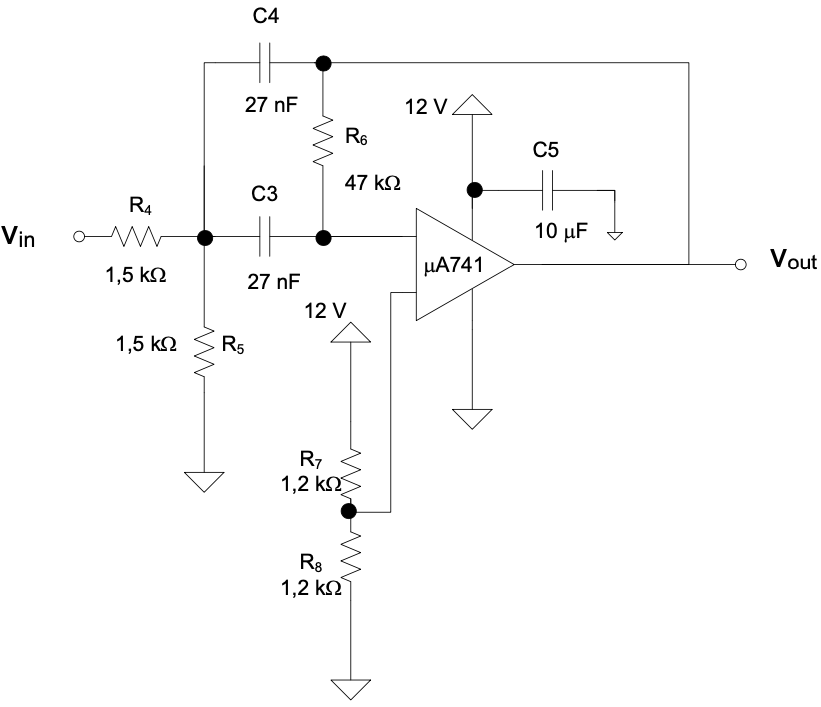
\includegraphics[width = 0.7 \textwidth]{Imagens/SecRauch.png}
    \caption{Esquema da montagem da secção biquadrática de Rauch.}
    \label{fig:passa_banda_Rauch} 
\end{figure}

\begin{figure}[ht]
    \centering
     \begin{subfigure}[b]{0.45\textwidth}
         \centering
         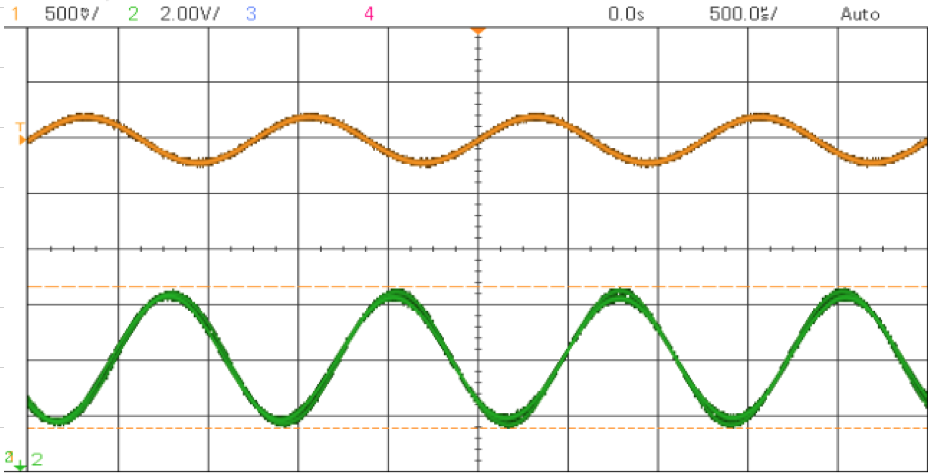
\includegraphics[width=\textwidth]{Imagens/fci.png}
         \caption{Entrada e saída do filtro para $f = 799$ Hz, obtendo-se $\Delta\phi = -135\degree$.}
     \end{subfigure}
     
     \begin{subfigure}[b]{0.45\textwidth}
         \centering
         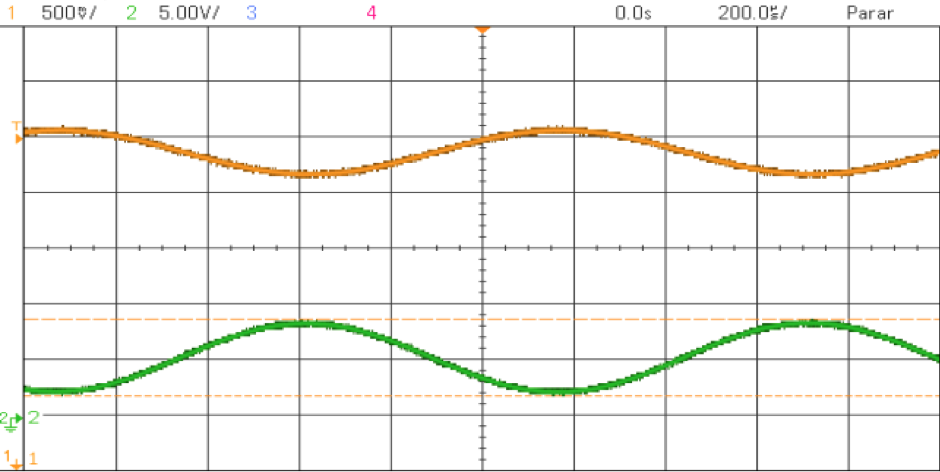
\includegraphics[width=\textwidth]{Imagens/f0.png}
         \caption{Entrada e saída do filtro para $f = 909$ Hz, obtendo-se $\Delta\phi = -179\degree$.}
     \end{subfigure}
     \begin{subfigure}[b]{0.45\textwidth}
         \centering
         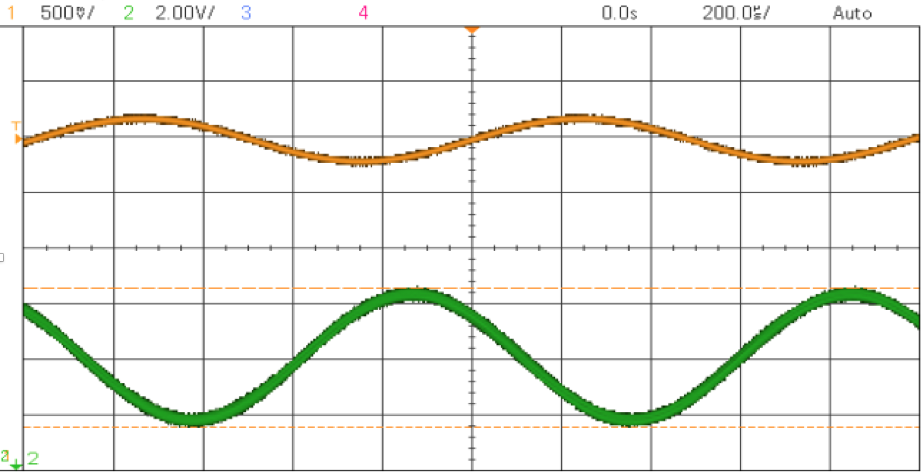
\includegraphics[width=\textwidth]{Imagens/fcs.png}
         \caption{Entrada e saída do filtro para $f = 1.03$ kHz, obtendo-se $\Delta\phi = 133\degree$.}
     \end{subfigure}
    \hfill
    \caption{Entrada e saída do filtro para vários valores de frequência.}
    \label{fig:ocsl_freqs}
\end{figure}

De seguida foi ligada a saída do oscilador à entrada do circuito atenuador, cujo esquema está apresentado na Fig. \ref{fig:atenuador}, e a sua saída ao filtro passa-banda. Na Fig. \ref{fig:breadbord} é apresentado o circuito montado no laboratório. O potenciómetro $\mathrm{P}_1$ foi ajustado de forma a não se verificar a saturação do AmpOp. Os resultados obtidos são apresentados na Fig. \ref{fig:res_ocl_atn_flt}.

\begin{figure}[h!]
    \centering
    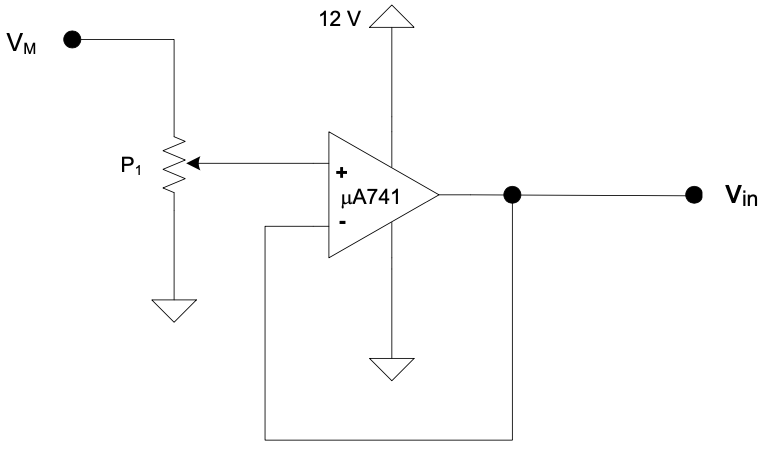
\includegraphics[width = 0.7 \textwidth]{Imagens/atenuador.png}
    \caption{Esquema do circuito atenuador.}
    \label{fig:atenuador}
\end{figure}

\begin{figure}[h!]
    \centering
    \includegraphics[width = 0.7 \textwidth]{Imagens/breadborad.pdf}
    \caption{Circuito montado no laboratório do sistema de deteção de distância a um obstáculo.}
    \label{fig:breadbord}
\end{figure}

\begin{figure}[h!]
    \centering
    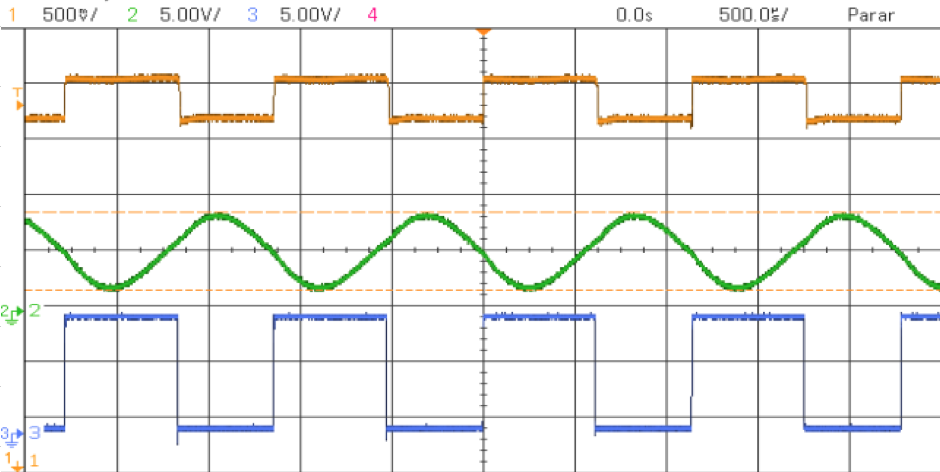
\includegraphics[width = 0.7 \textwidth]{Imagens/ocl_atn_flt.png}
    \caption{Resultados obtidos para a saída do oscilador (azul), atenuador (laranja), e passa-banda (verde).}
    \label{fig:res_ocl_atn_flt}
\end{figure}

\subsubsection{Comparação de Resultados}
Os resultados obtidos experimentalmente para as frequências de corte $f_{c_i}$ e $f_{c_s}$, frequência central do filtro $f_0$, largura de banda $B$, e ganho à frequência central $G_{f_0}$ são apresentados na Tabela \ref{tb:freqsRauch} e comparados com os valores obtidos na preparação teórica. Primeiro, é evidente que as frequências obtidas experimentalmente se encontram desfasadas em relação ao obtido na preparação teórica na direção das baixas frequências. Na verdade, este desfasamento da ordem de grandeza de 100Hz é idêntico para as três frequências medidas, como é verificável na semelhança dos valores dos erros relativos. O facto de ser idêntico sugere que a principal componente deste erro não advém de erros de medição, mas de desvios nas características dos elementos que compõem o filtro em relação às suas características nominais. Segundo, o valor obtido experimentalmente para a largura de banda é menor do que o previsto teoricamente. Para além do erro associado a desvios nas características dos elementos que compõem o filtro em relação às suas características nominais, o facto de este valor ter sido obtido a partir da subtração de dois valores obtidos experimentalmente (frequências de corte), cuja magnitude é uma ordem de grandeza acima, contribui também para um maior erro experimental. Terceiro, verificamos que o valor do ganho para a frequência central experimental é muito semelhante ao teórico obtido à frequência central teórica, tendo-se verificado um erro relativo reduzido.

\begin{table}[h!]
    \centering
    \caption{Comparação dos valores experimentais da frequência central e respetivo ganho, frequências de corte, e largura de banda com os obtidos na preparação teórica.}
    \begin{tabular}{cccc}
    \hline
    Parâmetro & Valor experimental & Valor teórico & Erro relativo \\
    \hline  
    $f_{c_i}$ & 799 Hz  &  875.0 Hz  & -8.87\%  \vspace{0.2cm} \\
    $f_{0}$& 909 Hz  & 1.000 kHz & -9.10\% \vspace{0.2cm} \\
    $f_{c_s}$& 1.03 kHz & 1.125 kHz & -8.44\% \vspace{0.2cm} \\
    $B$ &  231 Hz & 250.0 Hz & -7.60\% \vspace{0.2cm}\\
    $G_{f_0}$ & 23.4 dB  & 24.00 dB & -2.50 \%  \vspace{0.2cm}\\
    \hline
    \end{tabular}
    \label{tb:freqsRauch}
\end{table}

Finalmente, é possível analisar os resultados obtidos após a interconexão dos três circuitos montados na sessão 2 do trabalho laboratorial. Esta montagem tem como objectivo a determinação da distância entre o díodo e um recetor de IV, que foi modelado pelo circuito atenuador neste trabalho experimental. Assim, ao variar o valor da resistência do potenciómetro $\mathrm{P_1}$, está a simular-se a variação das perdas de energia do sinal com a distância ao longo do meio de transmissão entre o emissor de IV (díodo) e o recetor. Visto que a medição da onda diretamente do recetor de IV está contaminada com muito ruído numa larga gama de frequências, a filtragem do sinal com um filtro passa-banda permite selecionar uma banda restrita do sinal centrado numa frequência em que é sabido estar a ser transmitida a informação que permite inferir a distância entre o emissor e o recetor. Os resultados obtidos são apresentados na Fig. \ref{fig:res_ocl_atn_flt}. Primeiro, é possível notar o efeito da atenuação do sinal à saída do oscilador, comparando os sinais da saída do oscilador (azul) e da saída do atenuador (laranja). Notamos que como se trata de um andar de atenuação, o sinal de saída do atenuador tem a mesma forma à saída do oscilador. Segundo, notamos que à saída do filtro passa-banda a forma do sinal difere muito da forma à entrada do filtro. Este resultado é expectável, visto que a onda quadrada tem um espectro de frequência largo. De facto, é possível fazer a decomposição da onda quadrada em série de Fourrier, \textit{i.e.} numa combinação linear de sinusóides de frequência $f, 2f,... $, em que $f$ é a frequência do sinal $V_M$ calculada na Secção \ref{oscilador}. Note-se que $f\approx f_0$, \textit{i.e.} a frequência do sinal $V_M$ é idêntica à frequência central do filtro passa-banda determinada experimentalmente. Visto que o filtro é linear a sua saída pode ser interpretada como a soma da filtragem de cada uma das sinusóides individuais da série de Fourier. Desta forma, sabendo que o segundo termo da série ($2f \approx 2f_0$) é já atenuado em $\approx 30 $ dB em relação à sinusóide de frequência fundamental, a soma das sinusóides filtradas vai ser dominada pela sinusóide de frequência fundamental. Podemos verificar que os resultados da Fig.~\ref{fig:res_ocl_atn_flt} corroboram esta análise, visto que à saída do filtro observamos uma sinusóide quase perfeita de frequência $878$ Hz, o que corresponde a um erro relativo de $0.114$\% em relação à frequência determinada experimentalmente na Secção \ref{oscilador} para o sinal à saída do oscilador.

\subsubsection{Sugestão de melhoramento}
O desempenho do sistema de deteção de proximidade utilizado na sessão 2 desta atividade laboratorial pode ser melhorado de diversas formas. Primeiro, notamos que existe um desvio entre a frequência experimental do sinal à saída do oscilador e a frequência central do filtro passa-banda. Na verdade, considerando os valores experimentais do filtro-passa banda, conclui-se que existe uma atenuação de $\approx 6$dB na frequência experimental do oscilador em relação ao que seria obtido se as duas frequências coincidissem. Assim, deverá tentar-se regular os valores dos componentes em cada um dos circuitos por forma a alinhar as frequências experimentais. Na verdade, a substituição de uma das resistências $\mathrm{R_1}$ ou $\mathrm{R_2}$ por uma resistência variável permitiria fazer o ajuste da frequência da onda do oscilador experimentalmente de forma a coincidir com a frequência central do filtro. Segundo, por forma a obter uma filtragem mais restrita pode reduzir-se a largura de banda do filtro. Comparando \eqref{eq:tbp} com a função de transferência genérica de um filtro passa-banda de 2ª ordem obtém-se $B = \omega_0/Q$, pelo que para reduzir a largura de banda sem alterar o valor de $Q$ é necessário aumentar a frequência central do filtro passa-banda, por ajuste dos valores das resistências e dos condensadores que compõem o filtro. É de notar, que a frequência de saída do oscilador teria de ser ajustada para igualar a nova frequência central do filtro. Terceiro, visto que o objetivo é eliminar, o máximo possível, o ruído introduzido entre o emissor e o recetor de IV, aumentar a potência do emissor é uma opção que permite obter uma maior razão sinal-ruído à entrada do filtro passa-banda. Assim, diminuindo $\mathrm{R_3}$ até um valor próximo do valor mínimo calculado na Secção \ref{oscilador}, é possível aumentar a potência do sinal de IV irradiado pelo que será obtida uma menor razão sinal-ruído à saída do emissor. É, no entanto, expectável que o tempo de vida do díodo diminua com a implementação desta modificação.

\subsubsection{Conclusões}
A montagem da sessão tem como objectivo a determinação da distância entre o díodo e um recetor de IV, que foi modelado por um circuito atenuador neste trabalho experimental. Na verdade, o circuito atenuador simula as perdas de energia do sinal no meio de transmissão entre o emissor de IV (díodo) e o recetor. Visto que a medição da onda diretamente do recetor de IV está contaminada com muito ruído numa larga gama de frequências, a filtragem do sinal com um filtro passa-banda permite selecionar uma banda restrita do sinal centrado numa frequência em que é sabido estar a ser transmitida a informação que permite inferir a distância entre o emissor e o recetor. Em primeiro lugar, estudou-se um oscilador de onda retangular. Pôde observar-se os valores da frequência e do fator de ciclo tanto à saída do \textit{timer} ($V_M$) como à saída do condensador ($V_{C_1}$) e analisar a forma de onda de cada saída. Analisou-se ainda a corrente que atravessa o díodo do circuito, e foi calculada a resistência mínima $R_3$ que é possível selecionar para o bom funcionamento do díodo. Em segundo lugar, foi estudado o filtro passa-banda que corresponde a um filtro passa-banda de Butterworth de 2ª ordem. Foram feitos ensaios laboratoriais por forma a verificar os valores das frequências de corte $f_{c_i}$ e $f_{c_s}$, frequência central do filtro $f_0$, largura de banda $B$, e o ganho à frequência central $G_{f_0}$. Em terceiro lugar, foi construído e estudado o sistemas de deteção de distância, ligando a saída do oscilador à entrada do circuito atenuador e a sua saída ao filtro passa-banda. Notamos, que à saída do filtro passa-banda a forma do sinal difere muito da forma à entrada do filtro e que é gerada no oscilador. Na verdade, observamos uma sinusóide quase perfeita, um resultado que é expectável à luz da análise de Fourier da onda de entrada. Por fim, foram elencadas três alternativas por forma a aumentar o desempenho do sistema de deteção de proximidade: i) o alinhamento da frequência do oscilador e a frequência central do filtro passa-banda; ii) redução do ruído introduzido por redução da largura de banda do filtro; e iii) aumentar a relação sinal-ruído do sinal recebido através do aumento de potência do sinal que é emitido.